% ----------------------------------------------------------------
% AMS-LaTeX Paper ************************************************
% **** -----------------------------------------------------------
%\documentclass{amsart}
%\usepackage{txfonts}
%\documentclass[12pt,oneside]{article}
\documentclass{amsart}
\usepackage{graphicx}
\usepackage{enumitem}
% ----------------------------------------------------------------
\vfuzz2pt % Don't report over-full v-boxes if over-edge is small
\hfuzz2pt % Don't report over-full h-boxes if over-edge is small
% THEOREMS -------------------------------------------------------
\newtheorem{thm}{Theorem}[section]
\newtheorem{cor}[thm]{Corollary}
\newtheorem{lem}[thm]{Lemma}
\newtheorem{prop}[thm]{Proposition}
\theoremstyle{definition}
\newtheorem{defn}[thm]{Definition}
\theoremstyle{Exercise}
\newtheorem{ex}[thm]{Exercise}
\theoremstyle{remark}
\newtheorem{rem}[thm]{Remark}
\theoremstyle{rule}
\newtheorem{rul}[thm]{Rule}

\numberwithin{equation}{section}
% MATH -----------------------------------------------------------
\newcommand{\norm}[1]{\left\Vert#1\right\Vert}
\newcommand{\abs}[1]{\left\vert#1\right\vert}
\newcommand{\set}[1]{\left\{#1\right\}}
\newcommand{\Real}{\mathbb R}
\newcommand{\Z}{\mathbb Z}
\newcommand{\To}{\longrightarrow}
\newcommand{\BX}{\bB(X)}
\newcommand{\A}{\mathcal{A}}
% ----------------------------------------------------------------

% define some simple, commonly-used commands
\newcommand{\eps}{\varepsilon}
\newcommand{\dsum}{\displaystyle\sum}
\newcommand{\dint}{\displaystyle\int}

\newcommand{\pdr}[2]{\dfrac{\partial{#1}}{\partial{#2}}}
\newcommand{\pdrr}[2]{\dfrac{\partial^2{#1}}{\partial{#2}^2}}
\newcommand{\pdrt}[3]{\dfrac{\partial^2{#1}}{\partial{#2}{\partial{#3}}}}
\newcommand{\dr}[2]{\dfrac{d{#1}}{d{#2}}}
\newcommand{\aver}[1]{\langle {#1} \rangle}
\newcommand{\Baver}[1]{\Big\langle {#1} \Big\rangle}

\newcommand{\bzero}{\mathbf 0}
\newcommand{\bGamma}{\mbox{\boldmath{$\Gamma$}}}
\newcommand{\btheta}{\boldsymbol \theta}
\newcommand{\bchi}{\mbox{\boldmath{$\chi$}}}
\newcommand{\bnu}{\boldsymbol \nu}
\newcommand{\bmu}{\boldsymbol \mu}
\newcommand{\brho}{\mbox{\boldmath{$\rho$}}}
\newcommand{\bxi}{\boldsymbol \xi}
\newcommand{\bnabla}{\boldsymbol \nabla}
\newcommand{\bOm}{\boldsymbol \Omega}
\newcommand{\blambda}{\boldsymbol \lambda}
\newcommand{\bsigma}{\boldsymbol \sigma}

\newcommand{\bbR}{\mathbb R}
\newcommand{\bbC}{\mathbb C}
\newcommand{\bbQ}{\mathbb Q}
\newcommand{\bbN}{\mathbb N}
\newcommand{\bbZ}{\mathbb Z}

\newcommand{\ba}{\mathbf a} \newcommand{\bb}{\mathbf b}
\newcommand{\bc}{\mathbf c} \newcommand{\bd}{\mathbf d}
\newcommand{\be}{\mathbf e} \newcommand{\bff}{\mathbf f}
\newcommand{\bg}{\mathbf g} \newcommand{\bh}{\mathbf h}
\newcommand{\bi}{\mathbf i} \newcommand{\bj}{\mathbf j}
\newcommand{\bk}{\mathbf k} \newcommand{\bl}{\mathbf l}
\newcommand{\bm}{\mathbf m} \newcommand{\bn}{\mathbf n}
\newcommand{\bo}{\mathbf o} \newcommand{\bp}{\mathbf p}
\newcommand{\bq}{\mathbf q} \newcommand{\br}{\mathbf r}
\newcommand{\bs}{\mathbf s} \newcommand{\bt}{\mathbf t}
\newcommand{\bu}{\mathbf u} \newcommand{\bv}{\mathbf v}
\newcommand{\bw}{\mathbf w} \newcommand{\bx}{\mathbf x}
\newcommand{\by}{\mathbf y} \newcommand{\bz}{\mathbf z}
\newcommand{\bA}{\mathbf A} \newcommand{\bB}{\mathbf B}
\newcommand{\bC}{\mathbf C} \newcommand{\bD}{\mathbf D}
\newcommand{\bE}{\mathbf E} \newcommand{\bF}{\mathbf F}
\newcommand{\bG}{\mathbf G} \newcommand{\bH}{\mathbf H}
\newcommand{\bI}{\mathbf I} \newcommand{\bJ}{\mathbf J}
\newcommand{\bK}{\mathbf K} \newcommand{\bL}{\mathbf L}
\newcommand{\bM}{\mathbf M} \newcommand{\bN}{\mathbf N}
\newcommand{\bO}{\mathbf O} \newcommand{\bP}{\mathbf P}
\newcommand{\bQ}{\mathbf Q} \newcommand{\bR}{\mathbf R}
\newcommand{\bS}{\mathbf S} \newcommand{\bT}{\mathbf T}
\newcommand{\bU}{\mathbf U} \newcommand{\bV}{\mathbf V}
\newcommand{\bW}{\mathbf W} \newcommand{\bX}{\mathbf X}
\newcommand{\bY}{\mathbf Y} \newcommand{\bZ}{\mathbf Z}

\newcommand{\cA}{\mathcal A} \newcommand{\cB}{\mathcal B}
\newcommand{\cC}{\mathcal C} \newcommand{\cD}{\mathcal D}
\newcommand{\cE}{\mathcal E} \newcommand{\cF}{\mathcal F}
\newcommand{\cG}{\mathcal G} \newcommand{\cH}{\mathcal H}
\newcommand{\cI}{\mathcal I} \newcommand{\cJ}{\mathcal J}
\newcommand{\cK}{\mathcal K} \newcommand{\cL}{\mathcal L}
\newcommand{\cM}{\mathcal M} \newcommand{\cN}{\mathcal N}
\newcommand{\cO}{\mathcal O} \newcommand{\cP}{\mathcal P}
\newcommand{\cQ}{\mathcal Q} \newcommand{\cR}{\mathcal R}
\newcommand{\cS}{\mathcal S} \newcommand{\cT}{\mathcal T}
\newcommand{\cU}{\mathcal U} \newcommand{\cV}{\mathcal V}
\newcommand{\cW}{\mathcal W} \newcommand{\cX}{\mathcal X}
\newcommand{\cY}{\mathcal Y} \newcommand{\cZ}{\mathcal Z}


%%%%%%%%%%%%%%Start%%%%%%%%%%%%%Start%%%%%%%%%%%Start%%%%%%%%%%%%%%%Start%%%%%%%%%%%%%%%%%%%%%%%%%Start%%%%%%%%%%%%%%%%
%%%%%%%%%%%%%%Start%%%%%%%%%%%%%Start%%%%%%%%%%%Start%%%%%%%%%%%%%%%Start%%%%%%%%%%%%%%%%%%%%%%%%%Start%%%%%%%%%%%%%%%%
%%%%%%%%%%%%%%Start%%%%%%%%%%%%%Start%%%%%%%%%%%Start%%%%%%%%%%%%%%%Start%%%%%%%%%%%%%%%%%%%%%%%%%Start%%%%%%%%%%%%%%%%
%\documentclass[12pt,oneside]{article}

\usepackage{pdfpages}
%--------------
\usepackage{enumitem}
%-------------Tasks
%\usepackage{tasks} %\begin{tasks} \item \end{tasks}
%\bfseries Horizontal list: a = alphabetical \normalfont
%\begin{tasks}[counter-format = {tsk[a].},label-offset = {0.6em},label-format = {\bfseries}](6)
%\task One
%\task Two
%\task Three
%\task Four
%\task Five
%\task Six
%\task Seven
%\task Eight
%\task Nine
%\task Ten
%\end{tasks}
%\vglue5mm
%\bfseries Horizontal list: A = Alphabetical \normalfont
%\begin{tasks}[counter-format = {(tsk[A])},label-offset = {0.8em},label-format = {\bfseries}](3)
%\task One
%\task Two
%\task Three
%\task Four
%\task Five
%\task Six
%\task Seven
%\task Eight
%\task Nine
%\task Ten
%\end{tasks}



%___________________________
\usepackage[margin=2.5cm]{geometry}

\geometry{hmargin=3cm,vmargin=2cm}
\usepackage{tikz}
\def\width{18}
\def\hauteur{13}


\pagestyle{plain}

%%%%%%%%%%%%%%Start%%%%%%%%%%%%%Start%%%%%%%%%%%Start%%%%%%%%%%%%%%%Start%%%%%%%%%%%%%%%%%%%%%%%%%Start%%%%%%%%%%%%%%%%
%%%%%%%%%%%%%%Start%%%%%%%%%%%%%Start%%%%%%%%%%%Start%%%%%%%%%%%%%%%Start%%%%%%%%%%%%%%%%%%%%%%%%%Start%%%%%%%%%%%%%%%%
%%%%%%%%%%%%%%Start%%%%%%%%%%%%%Start%%%%%%%%%%%Start%%%%%%%%%%%%%%%Start%%%%%%%%%%%%%%%%%%%%%%%%%Start%%%%%%%%%%%%%%%%

\usepackage{fancyhdr}

\pagestyle{fancy}
\fancyhf{}
\rhead{}
\chead{\includegraphics[scale=.1]{snhu_logo.png}}
\begin{document}

\title{\sf MAT 230 Exam Two}%



%\thm{bbjh}


\begin{center}
\includegraphics[scale=.1]{snhu_logo.png}
\end{center}

%\thm{bbjh}
\maketitle
This document is proprietary to Southern New Hampshire University. It and the problems within may not be posted on any non-SNHU website.\\\\\\\\
\begin{center}
%Enter your name below this line:
Your Name Here
\end{center}

\begin{center}
\rule{\textwidth}{0.4pt}
\end{center}
\newpage
\section*{}
\section*{}
Directions: Type your solutions into this document and be sure to show all steps for arriving at your solution. Just giving a final number may not receive full credit.
\\
\section*{Problem 1}
 \noindent
 This question has 2 parts.
 \subsection*{Part 1:}
 Suppose that $F$ and $X$ are events from a common sample space with $P(F) \neq 0$ and $P(X) \neq 0$.
 \\
 \begin{enumerate}[label=(\alph*)]
     \item Prove that $P(X) = P(X|F)P(F) + P(X|\bar{F})P(\bar{F})$. Hint: Explain why $P(X|F)P(F) = P(X \cap F)$ is another way of writing the definition of conditional probability, and then use that with the logic from the proof of Theorem 4.1.1.
     \\\\
     %Enter your answer below this comment line.  
     \\\\
     \item Explain why $P(F|X) = P(X|F)P(F)/P(X)$ is another way of stating Theorem 4.2.1 Bayes’ Theorem.
     \\\\
     %Enter your answer below this comment line.  
     \\\\
 \end{enumerate}
 \subsection*{Part 2:}
 A website reports that 70\% of its users are from outside a certain country. Out of their users from outside the country, 60\% of them log on every day. Out of their users from inside the country, 80\% of them log on every day.
 \\
 \begin{enumerate}[label=(\alph*)]
 \item What percent of all users log on every day? Hint: Use the equation from Part 1 (a).
 \\\\
 %Enter your answer below this comment line.  
 \\\\
 \item Using Bayes’ Theorem, out of users who log on every day, what is the probability that they are from inside the country?
 \\\\
 %Enter your answer below this comment line.  
 \\\\
 \end{enumerate}
\newpage

~\\
  \section*{Problem 2}
 \noindent
 This question has 2 parts.
 \subsection*{Part 1:}
 The drawing below shows a Hasse diagram for a partial order on the set:
 \\
   $\{A, \;B,\; C,\; D,\; E,\; F,\; G,\; H,\; I, \; J\}$
 \begin{center}
 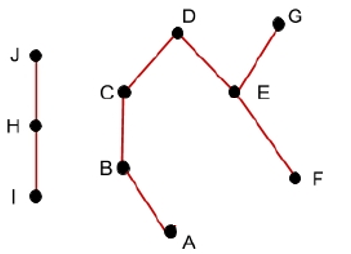
\includegraphics[width=2.5in]{NewHasse}
 \end{center}
 {\color{blue} {\bf Figure 1:} \emph{A Hasse diagram shows 10 vertices and 8 edges. The vertices, represented by dots, are as follows:  vertex J is upward of vertex H; vertex H is upward of vertex I; vertex B is inclined upward to the left of vertex A; vertex C is upward of vertex B; vertex D is inclined upward to the right of vertex C; vertex E is inclined upward to the left of vertex F; vertex G is inclined upward to the right of vertex E. The edges, represented by line segments between the vertices are as follows: 3 vertical edges connect the following vertices: B and C, H and I, and H and J; 5 inclined edges connect the following vertices: A and B, C and D, D and E, E and F, and E and G. 
  }
  }
  \\\\
 Determine the properties of the Hasse diagram based on the following questions:

  \begin{enumerate}[label=(\alph*)]
    \item What are the minimal elements of the partial order?
\\\\
  %Enter your answer below this comment line.  
\\\\
    \item What are the maximal elements of the partial order?
\\\\
  %Enter your answer below this comment line.  
\\\\
    \item Which of the following pairs are comparable?
\[(A,\, D),\; (J,\, F),\; (B,\, E),\; (G,\, F),\; (D,\, B),\; (C,\, F),\; (H,\, I), (C,\, E)\]
\\\\
  %Enter your answer below this comment line.  
\\\\
   \end{enumerate}
   \newpage
~\\
\subsection*{Part 2:}
Consider the partial order with domain $\{3,\, 5,\, 6, \,7,\, 10,\, 14,\, 20,\, 30,\, 60,\, 70\}$ and with $x\,\leq \,y$ if $x$ evenly divides $y$. Select the correct Hasse diagram for the partial order.

\begin{enumerate}[label=(\alph*)]
\item
\fbox{
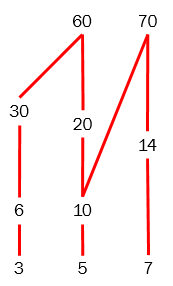
\includegraphics[height=3in]{Figure2}\\

}
\\\\
{\color{blue}{\bf Figure 2:} \emph{A Hasse diagram shows a set of elements {3; 5; 6; 7; 10; 14; 20; 30; 60, 70}. There are lines connecting 3 and 6, 6 and 30, 30 and 60, 5 and 10, 10 and 20, 20 and 60, 10 and 70, 7 and 14, 14 and 70.
}
}
\\
\\
  %Enter your answer below this comment line.  
\\\\
\newpage
~\\~\\
\item
\fbox{
 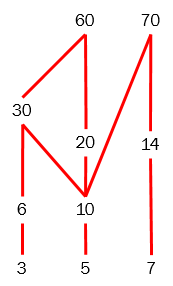
\includegraphics[height=3in]{Figure3}
}
\\\\
{\color{blue}{\bf Figure 3:} \emph{A Hasse diagram shows a set of elements {3; 5; 6; 7; 10; 14; 20; 30; 60, 70}. There are lines connecting 3 and 6, 6 and 30, 30 and 60, 5 and 10, 10 and 30, 10 and 20, 20 and 60, 10 and 70, 7 and 14, 14 and 70.
}
}
\\
\\
  %Enter your answer below this comment line.  
\\\\
\newpage
~\\~\\
\item
\fbox{
 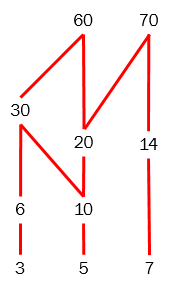
\includegraphics[height=3in]{Figure4}\\
}
\\\\
{\color{blue}{\bf Figure 4:} \emph{A Hasse diagram shows a set of elements {3; 5; 6; 7; 10; 14; 20; 30; 60, 70}. There are lines connecting 3 and 6, 6 and 30, 30 and 60, 5 and 10, 10 and 30, 10 and 20, 20 and 60, 20 and 70, 7 and 14, 14 and 70.
}
}
\\
\\
  %Enter your answer below this comment line.  
\\\\
\newpage
~\\~\\
\item
\fbox{
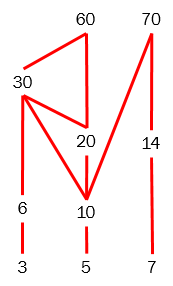
\includegraphics[height=3in]{Figure5}
}
\\\\
{\color{blue}{\bf Figure 5:} \emph{A Hasse diagram shows a set of elements {3; 5; 6; 7; 10; 14; 20; 30; 60, 70}. There are lines connecting 3 and 6, 6 and 30, 30 and 60, 5 and 10, 10 and 30, 10 and 20, 20 and 30, 20 and 60, 10 and 70, 7 and 14, 14 and 70.
}
}
\\\\
  %Enter your answer below this comment line.  
\\\\

\end{enumerate}
  \newpage
~\\
  \section*{Problem 3}
  A car dealership sells cars that were made in 2015 through 2020. Let the cars for sale be the domain of a relation R where two cars are related if they were made in the same year.

  \begin{enumerate}[label=(\alph*)]
    \item Prove that this relation is an equivalence relation.
\\\\
  %Enter your answer below this comment line.  
\\\\
    \item Describe the partition defined by the equivalence classes.
\\\\
  %Enter your answer below this comment line.  
\\\\
  \end{enumerate}
\newpage
~\\
  \section*{Problem 4}
 Analyze each graph below to determine whether it has an Euler circuit and/or an Euler trail.
 \begin{itemize}
     \item If it has an Euler circuit, specify the nodes for one.
     \item If it does not have an Euler circuit, justify why it does not.
     \item If it has an Euler trail, specify the nodes for one.
     \item If it does not have an Euler trail, justify why it does not.
 \end{itemize}
  \begin{enumerate}[label=(\alph*)]
\item 
\fbox{
 
\includegraphics[width=4in]{Figure6}
}
\\\\
{\color{blue} {\bf Figure 6:} \emph{An undirected graph has 6 vertices, a through f. There are 8-line segments that are between the following vertices: a and b, a and c, a and d, a and f, b and c, b and e, b and f, d and e. 
  }
}\\\\
  %Enter your answer below this comment line.  
\\\\
   \newpage
~\\~\\
\item
\fbox{
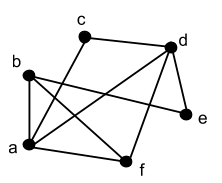
\includegraphics[width=4in]{Figure7}
}
\\\\
{\color{blue} {\bf Figure 7:} \emph{
An undirected graph has 6 vertices, a through f. There are 9-line segments that are between the following vertices: a and b, a and c, a and d, a and f, b and e, b and f, c and d, d and e, d and f. }
}
\\\\
  %Enter your answer below this comment line.  
\\\\
   \newpage
~\\~\\
\item 
\fbox{
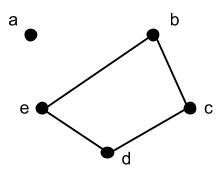
\includegraphics[width=4in]{Figure8}
}
\\\\
{\color{blue} {\bf Figure 8: } \emph{An undirected graph has 5 vertices, a through e. There are 4-line segments that are between the following vertices: b and c, b and e, c and d, d and e. 
  }
}
\\\\
  %Enter your answer below this comment line.  
\\\\

\newpage
~\\~\\
\item 
\fbox{
 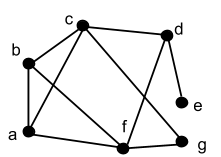
\includegraphics[width=4in]{Figure9}
}
\\\\
{\color{blue} {\bf Figure 9:} \emph{An undirected graph has 7 vertices, a through g. There are 10-line segments that are between the following vertices: a and b, a and c, a and f, b and c, b and f, c and d, c and g, d and e, d and f, f and g. 
  }
}
\\\\
  %Enter your answer below this comment line.  
\\\\


  \end{enumerate}
\newpage
~\\
  \section*{Problem 5}
  Use Prim's algorithm to compute the minimum spanning tree for the weighted graph. Start the algorithm at vertex A. Explain and justify each step as you add an edge to the tree.
\\
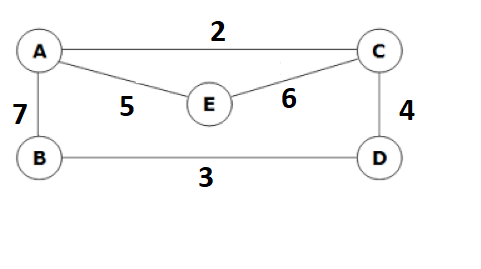
\includegraphics[width=5in]{prim}
\\\\
{\color{blue} {\bf Figure 10:} \emph{A weighted graph shows 5 vertices, represented by circles, and 6 edges, represented by line segments. Vertices A, B, C, and D are placed at the corners of a rectangle, whereas vertex E is at the center of the rectangle. The edges, A B, B D, A C, C D, A E, and E C, have the weights, 7, 3, 2, 4, 5, and 6, respectively.
  }
}
\\\\
  %Enter your answer below this comment line.  
\\\\
 \newpage
~\\
  \section*{Problem 6}
A lake initially contains 1000 fish. Suppose that in the absence of predators or other causes of removal, the fish population increases by 10\% each month. However, factoring in all causes, 80 fish are lost each month.\\

Give a recurrence relation for the population of fish after $n$ months. How many fish are there after 5 months? If your fish model predicts a non-integer number of fish, round down to the next lower integer.
\\\\
  %Enter your answer below this comment line.  
\\\\
\end{document}

